% !TEX root = www2019-visual-ltr.tex

\section{\protect\modelname{} Model}
In this section, we introduce the \modelname{} model for \ac{LTR} with visual features.
The proposed model consists of three parts.
First, we introduce the model architecture in Section~\ref{sec:multimodal}.
Then, in Section~\ref{sec:visualfeatures} we describe two visual feature extractors used by \modelname{}:
VGG-16~\cite{simonyan2014very} and ResNet-152~\cite{he2016deep}, both pretrained on ImageNet.
Finally, in Section~\ref{sec:saliency} we propose to enhance \modelname{} by generating synthetic saliency heatmaps for each of the input images.
%These synthetic saliency images are trained to learn a more expressive representation of the viewing pattern of a user. 
 The implementation of the proposed \modelname{} model is available at \url{http://anonymized.url}.

\subsection{Architecture} \label{sec:multimodal}
%In order to compare the performance of various visual feature extractor methods, we propose a reusable multimodal architecture. 
The \modelname{} architecture is visualized in Figure~\ref{fig:multimodelarchitecture}. 
The model starts by taking an image $x_i$ (1) as an input to the visual feature extraction layer (2) in order to create a generic visual feature vector $x_{vf}$. 
These features are considered generic because they can be extracted by using a convolutional filters that were trained on a different dataset and task. 
In order to transform these $x_{vf}$ to an \ac{LTR} specific visual feature vector, we use $x_{vf}$ as an input to the visual feature transformation layer.
This visual feature transformation layer is optimized to convert generic visual features to a visual feature vector $x_{vl}$ such that they can be used in combination with other \ac{LTR} features. 

Separating the visual feature extraction and feature transformation layers allows us to significantly reduce the computation requirements when using a pre-trained model for visual feature extraction. 
In Section ~\ref{sec:sectionoptimalization} we further elaborate how the computational requirements can be reduced. In Section~\ref{sec:visualfeatures} we demonstrate how transfer-learning can be applied to use pre-trained models in combination with the \modelname{} architecture.

The \modelname{} architecture also makes use of content features $x_{c}$ (4), e.g., BM25, PageRank, etc.
The final feature vector $x_{l}$ is constructed by concatenating the visual features $x_{vl}$ with the content features~$x_{c}$.
%
This final feature vector $x_{l}$ is then used as an input to the scoring component (5),
which transforms the features into a single score $x_s$ for each query-document pair.
The resulting model is trained end-to-end using a pairwise hinge loss with $L_2$ regularization similarly to~\cite{fan2017learning}.
The scoring component uses a single fully connected layer with a hidden size of $10$ and dropout set to $10\%$,
which showed good performance in preliminary experiments.

% \begin{multline}
% x_{vl} = f_{t}(f_{v}(x_{v})) \\ x_{s} = f_{s}(x_{vl} \oplus x_{c}) 
% \end{multline}


\begin{figure}[t]
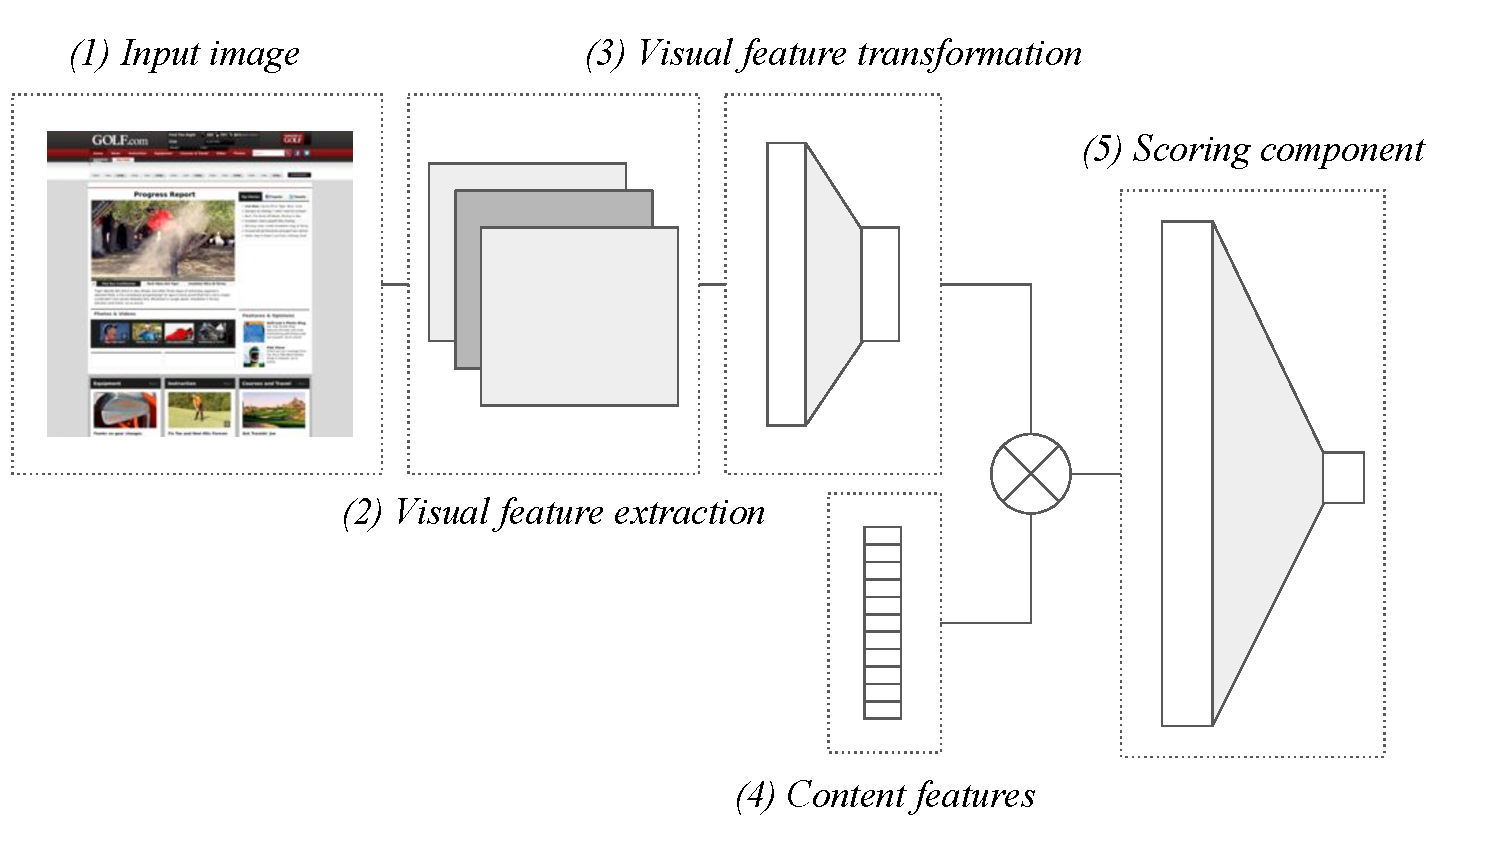
\includegraphics[width = 3.4in]{images/multimodelarchitecture.pdf}
\caption{\modelname{} architecture.}
\label{fig:multimodelarchitecture}
\end{figure}

\subsection{Visual Feature Extractors} \label{sec:visualfeatures}
In order to use the webpage snapshots in \ac{LTR}, the snapshots have to be transformed to a vector representation that can be used in combination with existing content features. 
Because the amount of training examples in \datasetname{} is relatively low, it is beneficial to use a model that was pre-trained on a large image dataset and for a different task, eg. image classification. Convolutional filters generalize well and are easily transferable to other tasks.  In this work we use the VGG-16~\cite{simonyan2014very} and ResNet-152~\cite{he2016deep} models, two well-explored image classification models which both have an implementation with ImageNet pre-trained parameters available for PyTorch. The two paragraphs below describe how these two models are implemented within the \modelname{} architecture.




% Since our introduced \datasetname{} data\-set has a relatively low number of snapshots to train a separate feature extractor, we use the VGG-16~\cite{simonyan2014very} and ResNet-152~\cite{he2016deep} models pretrained on ImageNet as two separate feature extractors.
% \todo{Change the story: (1) we need visual feature extractors, (2) the amount of training data is usually low, so it is better to pretrain, (3) say something about the state-of-the-art, i.e., how novel and up-to-date these methods are.}

VGG-16~\cite{simonyan2014very} is commonly used for training transfer-learned models,
because it provides a reasonable trade-off between effectiveness and simplicity~\cite{shan2017two}.
The VGG-16 architecture consists of a set of convolutional layers and fully connected layers. 
The convolutional layers extract features from an input image, which are then used by the fully connected layers to classify the image. 
The convolutional layers of VGG-16 are generic with respect to an input and task~\citep{donahue2014decaf}
and, thus, can be used as a visual feature extractor within the \modelname{} architecture to create generic visual features $x_{vf}$.
For this reason, we use the convolutional layers as is, by freezing all the parameters during training.
The fully connected layers of VGG-16, instead, can be altered and retrained in order to be used with new inputs and tasks.
Due to this, we utilize them as a visual feature transformation layer within the \modelname{} architecture to produce \ac{LTR} specific features $x_{vl}$.
In particular, we replace the last fully connected layer of VGG-16 by a newly initialized fully connected layer.
Then we optimize the parameters of all fully connected layers of VGG-16 during training.
The size of $x_{vl}$ is set to $30$, as this size showed good performance in preliminary experiments.

The ResNet-152~\cite{he2016deep} architecture was shown to outperform VGG-16 in ImageNet classification.
The residual connections between convolutional layers of ResNet-152 allow for deeper networks to be trained without suffering from vanishing gradients.
Similarly as VGG-16, ResNet-152 has convolutional layers that extract features from the input images, which are in turn used by a fully connected layer to classify each image.
We use these convolutional layers as the visual feature extraction layer, which transforms $x_{i}$ to $x_{vf}$. All parameters of these convolutional layers are frozen during training.

Other than VGG-16, the original ResNet-152 architecture only has a single fully connected layer, which empirically showed to not be enough to successfully train the model.
Instead, we transform $x_{vf}$ to $x_{vl}$ by training a fully connected network from scratch.
The transformation layer is constructed using three layers with each $4096$ hidden units and a final layer resulting in $x_{vl}$ with a size of $30$, which was empirically found to provide good performance in preliminary experiments.


\subsection{Saliency Heatmaps} \label{sec:saliency}
In order to increase the ability to learn the visual quality of a webpage, we propose to explicitly model the user viewing pattern through synthetic saliency heatmaps.
The use of saliency heatmaps could be advantageous compared to the use of raw snapshots for the following reasons.
First, synthetic saliency heatmaps explicitly learn to predict how users perceive webpages by training an end-to-end model on actual eye-tracking data.
We expect this information to better correlate with webpage relevance compared to raw snapshots.
Second, saliency heatmaps reduce the average storage requirements by up to 90\%,
because they are gray-scale images and have large areas of the same color, which can be stored efficiently.
This makes the use of saliency heatmaps attractive for practical applications.
Figure~\ref{fig:exampleshots} shows example snapshots with their corresponding heatmaps (first and third columns respectively).

Following \cite{shan2017two}, we use a two-stage transfer learning model that learns how to predict saliency heatmaps on webpages.
Similarly to the visual feature extraction approaches above, \cite{shan2017two} takes a pre-trained image recognition model and finetunes the output layers on the following two datasets in order respectively:
\begin{inparaenum}[(i)]
\item SALICON~\cite{jiang2015salicon}, a large dataset containing saliency heatmaps created with eye-tracking hardware on natural images, and 
\item the webpage saliency dataset from \cite{shen2014webpage}, a smaller dataset containing saliency heatmaps created with eye-tracking hardware on webpages.
\end{inparaenum}

The trained model is used to convert a raw snapshot into a synthetic saliency heatmap. This heatmap is then used as an input image $x_i$ for the \modelname{} model (see Figure~\ref{fig:multimodelarchitecture}).

\if0
The trained model is applied to the $3\times224\times224$ input images \todo{where do such images come from?}, resulting in grayscale heatmaps with a dimension of $1\times64\times64$.
\todo{Does this model always reduce the dimension size by 3?}
These heatmaps are then used as the an input image $x_{v}$ for the visual feature extractors described above (see Figure~\ref{fig:multimodelarchitecture}) by linearly scaling them to $3\times224\times224$, matching them with the VGG-16 and ResNet-152 input dimensions.
\fi